\section{Utilization}

The utilization chapter goes through a specific use case, explains in detail how to use the tool and the output it produces. It furthers talks about limitations and aspects in regards to perfomance. 

\subsection{Use Cases}

\textbf{Scenario}: The user wants to run the static analysis on a Linux machine and have the results displayed on the console.

\subsection{Execution: Step-by-step Guide}

Here is a step by step discription how the use case is played out.

\subsubsection{Open terminal and execute Python package}

It is a CLI tool and therefore it is mandatory to use the terminal for the tool to work. Once everything is set up properly the tool is run by writing "linux-analyzer" on the command line and pressing enter.

\smallskip
\begin{figure}[h]
\centering
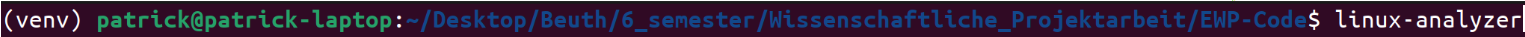
\includegraphics[scale=0.3, keepaspectratio]{images/linux-analyzer-cmd-line-exec}
\caption{Tool Execution - Command Line}
\end{figure}

If everything works and the tool starts up properly a prompt will be visible next. It asks the user to choose a mode for the analysis and if applicable the report or/and cve option.

\smallskip
\begin{figure}[h]
\centering
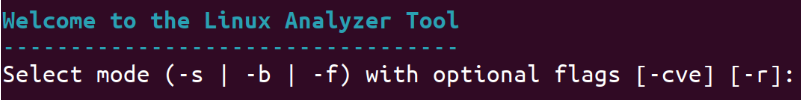
\includegraphics[scale=0.3, keepaspectratio]{images/user-input-prompt}
\caption{Prompt for user input}
\end{figure}

After picking the flags the program runs with the chosen settings.\newline Insert pick during runtime!


\subsection{Output Interpretation}

The output of the analysis is displayed on the console as the default configuration. The user can use the optional -r flag when executing the tool to generate a report in text file format. \newline The content and meaning of the ouput is dependent on the mode and optional flags chosen by the user. 

\subsubsection{Example Outputs}

\subsection{Limitations in Usage}

There are certain limitations in place. It is a CLI tool, therefore it has to be started from the command line. This is non-negotiable and the only way to use the tool. \newline The tool solely runs on machines which have a Linux distribution as there operating system.

\subsubsection{Permissions and Rights}

The tool handles highly sensitive data. This is why getting the permissions and rights exactly right is of paramount importance. Consequently running the entire tool with root privileges is out of question. The goal is to have a nuanced approach and identify the exact areas and which need elevated privileges. This scenario calls for the security design principle referred to as privilege separation. Each component of the application has tailored and distinct privileges according to its needs and tasks. No component has more privileges than it needs to do its designated jobs.\newline 

The static analysis does not need root privileges. It needs read access to files and certain folders including \textit{/user/bin}, \textit{/etc} among others. It may need elevated read access on hardened systems but is can be solved through group membership, read-only ACLs and capabilities.\newline 

The behavioral part of the analysis is a different story though. Runtime analysis requires root or near-root privileges in regards to syscall tracing, eBPF, network inspection and kernel/process introspection. It is important to note that some will run as actual root while others will use a dedicated system user with specific capabilities whenever possible.

\subsection{Performance}

\subsubsection{Execution Time}

\subsubsection{Statisitcs and Benchmarking}